\documentclass[tikz,border=3mm]{standalone}
\usepackage[T1]{fontenc}
\usepackage[utf8]{inputenc}
\usepackage{lmodern}
\usetikzlibrary{arrows.meta,positioning,calc,shapes.geometric}
\definecolor{ink}{HTML}{202A33}
\definecolor{blue}{HTML}{2D7F9D}
\definecolor{orange}{HTML}{C97728}
\definecolor{light}{HTML}{B0C0D0}
\definecolor{soft}{HTML}{F3F5F7}
\begin{document}
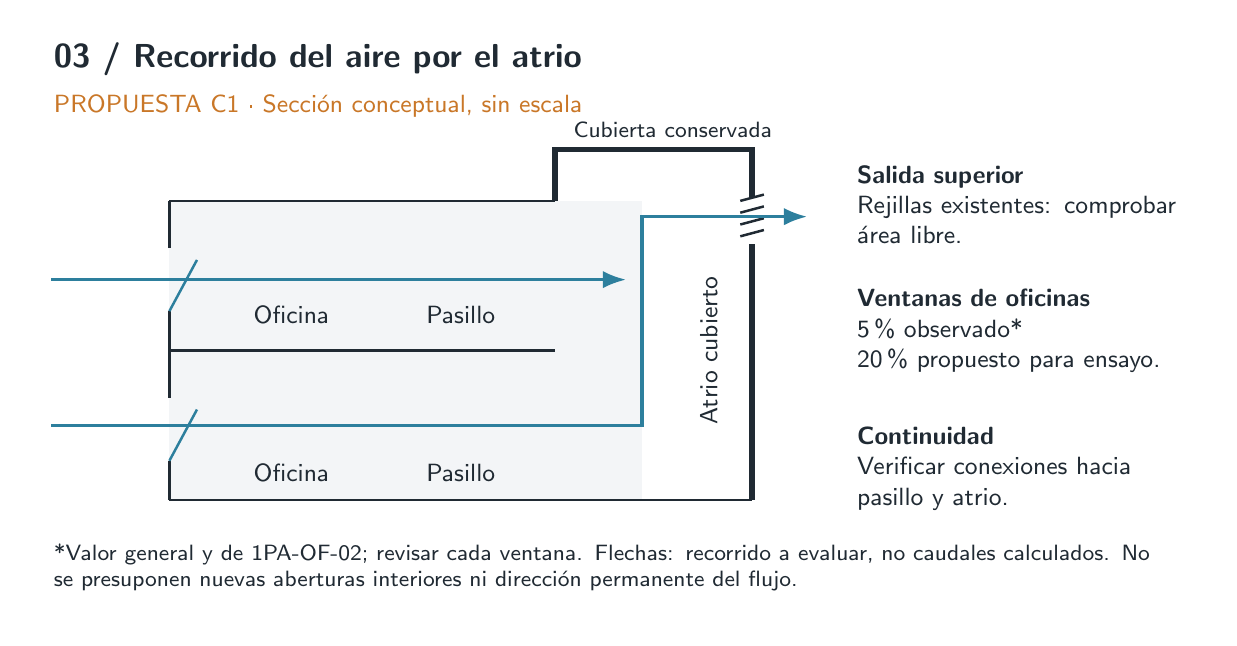
\begin{tikzpicture}[x=1cm,y=1cm,>=Latex,line width=.9pt,every node/.style={font=\sffamily\small,text=ink},note/.style={align=left,text width=4.1cm,anchor=west},flow/.style={->,blue,line width=1.2pt}]
\path[use as bounding box] (0,0) rectangle (15,7.5);

\node[anchor=west,font=\sffamily\bfseries\large] at (.2,7.1) {03 / Recorrido del aire por el atrio};
\node[anchor=west,text=orange] at (.2,6.5) {PROPUESTA C1 · Sección conceptual, sin escala};
\fill[soft] (1.8,1.5) rectangle (7.8,5.3);
\draw[ink] (1.8,1.5)--(9.2,1.5) (1.8,3.4)--(6.7,3.4) (1.8,5.3)--(6.7,5.3);
\draw[ink,line width=2pt] (6.7,5.3)--(6.7,5.95)--(9.2,5.95)--(9.2,5.35) (9.2,4.75)--(9.2,1.5);
\draw[ink] (1.8,1.5)--(1.8,2) (1.8,2.8)--(1.8,3.9) (1.8,4.7)--(1.8,5.3);
\draw[blue] (1.8,2)--(2.15,2.65) (1.8,3.9)--(2.15,4.55);
\foreach \y in {4.85,5,5.15,5.3} \draw[ink] (9.05,\y)--(9.35,\y+.08);
\draw[flow] (.3,2.45)--(3.1,2.45)--(5.5,2.45)--(7.8,2.45)--(7.8,5.1)--(9.9,5.1);
\draw[flow] (.3,4.3)--(3.1,4.3)--(5.5,4.3)--(7.6,4.3);
\node at (3.35,3.85) {Oficina}; \node at (5.5,3.85) {Pasillo};
\node at (3.35,1.85) {Oficina}; \node at (5.5,1.85) {Pasillo};
\node[rotate=90] at (8.65,3.4) {Atrio cubierto};
\node[anchor=west,font=\sffamily\footnotesize] at (6.8,6.2) {Cubierta conservada};
\node[note] at (10.4,5.25) {\textbf{Salida superior}\\Rejillas existentes: comprobar área libre.};
\node[note] at (10.4,3.65) {\textbf{Ventanas de oficinas}\\5\,\% observado*\\20\,\% propuesto para ensayo.};
\node[note] at (10.4,1.9) {\textbf{Continuidad}\\Verificar conexiones hacia pasillo y atrio.};
\node[anchor=west,text width=14cm,align=left,font=\sffamily\footnotesize] at (.2,.65) {*Valor general y de 1PA-OF-02; revisar cada ventana. Flechas: recorrido a evaluar, no caudales calculados. No se presuponen nuevas aberturas interiores ni dirección permanente del flujo.};

\end{tikzpicture}
\end{document}
